\documentclass[aspectratio=1610]{beamer}

\usetheme{unnslides}
\usefonttheme{professionalfonts}

\usepackage{listings}
\usepackage{graphicx}
\usepackage{caption}
\usepackage{cmbright}
\usepackage{fontspec}
\usepackage{unicode-math}
\usepackage{amsfonts}
\usepackage{subfig}

\setromanfont{CMU Serif}
%\setsansfont{CMU Sans Serif}
\setmathfont{Latin Modern Math}

\usepackage{polyglossia}
%\setbeamertemplate{itemize item}{\color{black}$\blacktriangleright$}

\DeclareMathOperator*{\argmax}{arg\,max}
\DeclareMathOperator*{\argmin}{arg\,min}
\DeclareMathOperator{\sign}{sign}
\DeclareMathOperator{\re}{Re}

\graphicspath{ {../paper/images/}{img/} }
%set pages numeration
\setbeamertemplate{footline}[frame number]
\setbeamertemplate{headline}{}
\setlength\abovecaptionskip{-1pt}

\title{Comparison of dimensionality reduction schemes for derivative-free global optimization algorithms}
\author{\textbf{Vladislav~Sovrasov}}
\institute{Lobachevsky State University of Nizhni Novgorod}
\date{}

\begin{document}
\begin{frame}[noframenumbering,plain]
\titlepage
\end{frame}

\begin{frame}
  \begin{center}
  \frametitle{Problem statement}

  \begin{displaymath}
    \min\{f(y): y\in D\}, D=\{y\in \mathbb{R}^n: a_i \leqslant y_i \leqslant b_i, 1\leqslant i \leqslant n \},
  \end{displaymath}
where \(f(y)\) is a vector-function.

\enspace
Solution of the problem is a set of non-dominated points (Slater set):
  \begin{displaymath}
    S(D) = \{y\in D: \nexists z\in D, f_i(z)<f_i(y),1\leqslant i \leqslant m\}
  \end{displaymath}
Assume objectives to satisfy Lipschitz condition in \(D\):
  \begin{displaymath}
    |f_i(y_1)-f_i(y_2)|\leqslant L_i\Vert y_1-y_2\Vert,y_1,y_2\in D,0<L_i<\infty,1\leqslant i\leqslant m
  \end{displaymath}

\end{center}
\end{frame}

\begin{frame}
  \frametitle{Dimension reduction}
  Peano-type curve \(y(x)\) allows to reduce dimension of the original multi-objective problem:
  \begin{gather}
    \lbrace y\in \mathbb{R}^N:-2^{-1}\leqslant y_i\leqslant 2^{-1},1\leqslant i\leqslant N\rbrace=\{y(x):0\leqslant x\leqslant 1\} \nonumber \\
    \min\{f(y): y\in D\}=\min\{f(y(x)): x\in [0,1]\} \nonumber
  \end{gather}

  %\begin{figure}[ht]
  %  \subfloat{{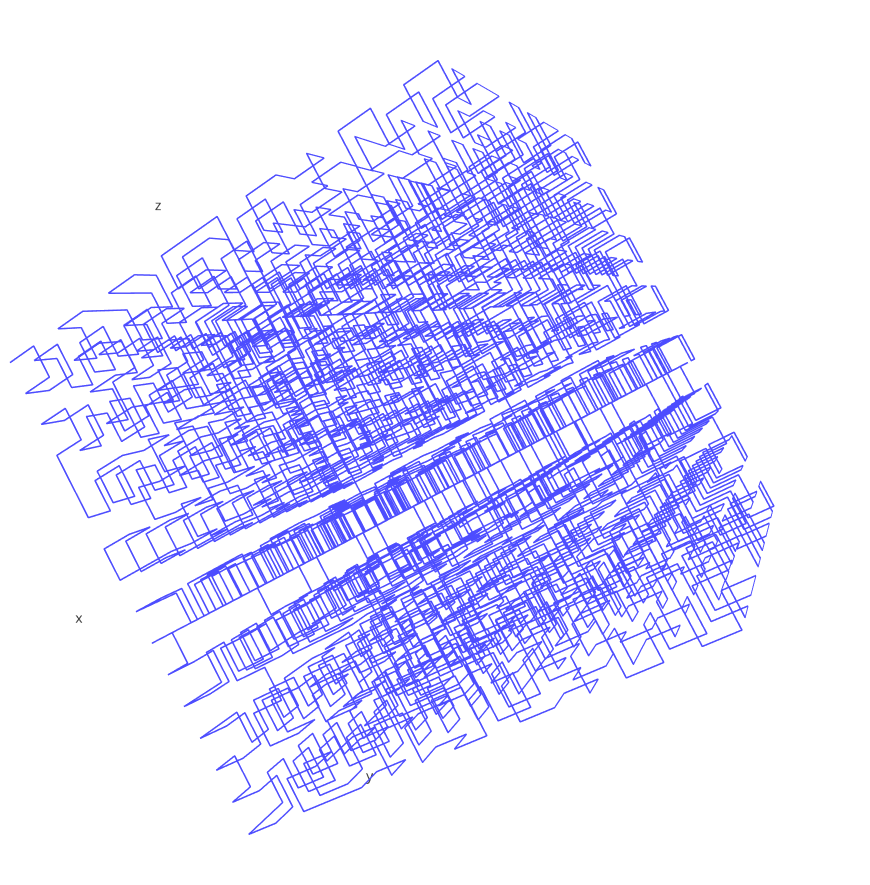
\includegraphics[width=.35\textwidth]{img/peano3d.png} }}
  %  \subfloat{{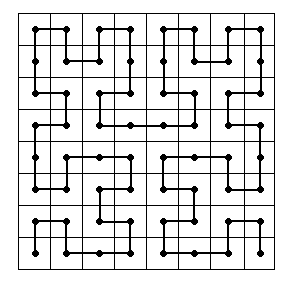
\includegraphics[width=.35\textwidth]{img/peano2d.png} }}
  %\end{figure}
\end{frame}

\begin{frame}
  \frametitle{Conclusion and future work}
    Already done:
    \begin{itemize}
      \item
    \end{itemize}
    Future work:
    \begin{itemize}
      \item
    \end{itemize}
\end{frame}

\begin{frame}{{}}
  \frametitle{ }
  \begin{center}
    \Large{Q\&A}

\vspace{1cm}

    sovrasov.vlad@gmail.com

    https://github.com/sovrasov
  \end{center}
\end{frame}

\end{document}
